\section{Agricultural Robots}

	Agricultural robots are designed to be implemented on an unstructured environment. Hence, these robots are expected to be dynamic, uncertain, complex, highly variable, and hostile. In order to build an agricultural robot, multiple design principles are taken into consideration. This includes product specification such as speed, system analysis such as the function, concept development such as alternative methods, feasibility, and what not. Figure~\ref{fig:robot} shows the flowchart  of the implementation of concepts on an agricultural robot.~\cite{Edan}

\begin{figure}[!b]
	\centering
		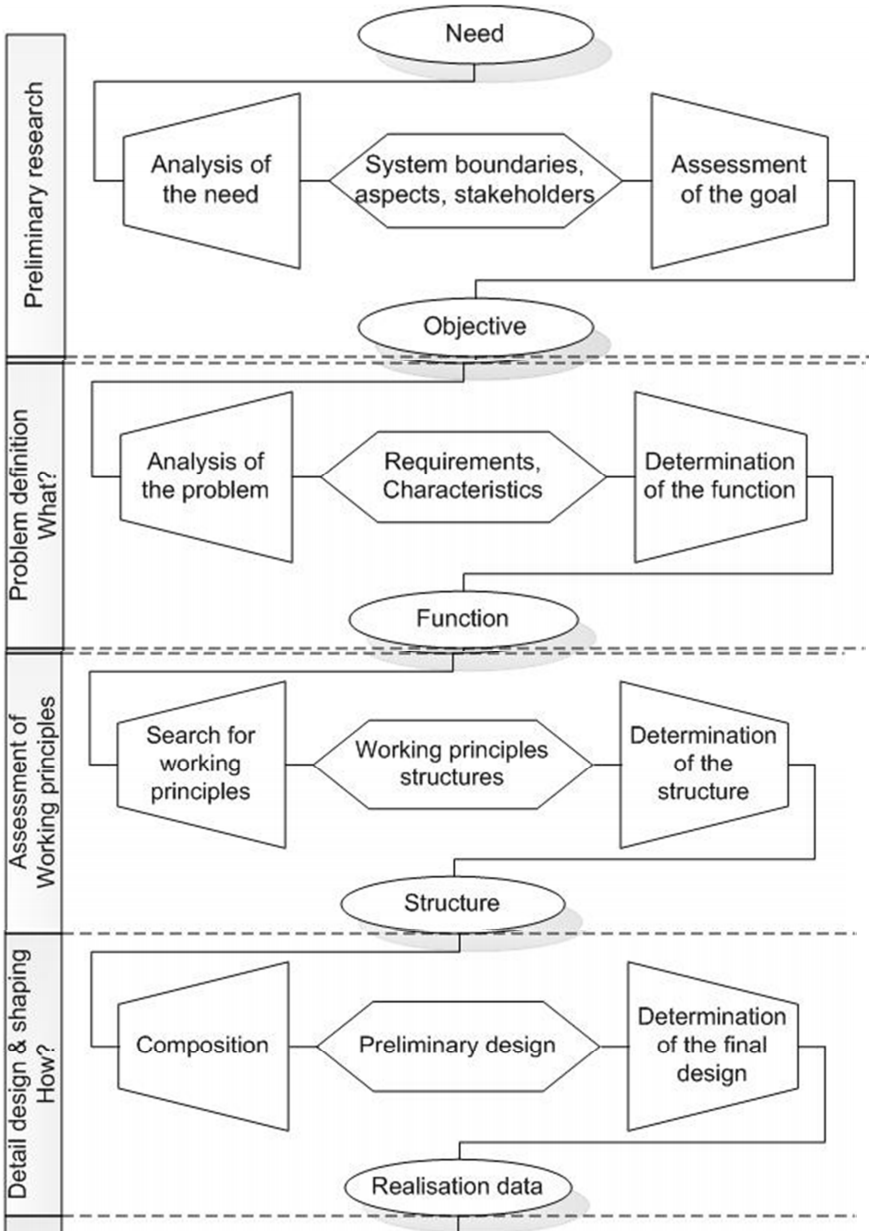
\includegraphics[width=2.5 in]{robot}
	\caption{Flowchart of Agricultural Robot Design}
	\label{fig:robot}
\end{figure}

\section{Raspberry Pi 3 Model B}

	Raspberry Pi is a low-cost microcomputer originally designed to aide young people in programming. It is advantageous in terms of size, portability, cost, programmability, and connectivity.~\cite{vid} Raspberry Pi is mounted on a credit card-sized board and has multiple feature ports such as USB 2.0, HDMI, Power, SD Card, and many more depending on the model.

	On this research, Raspberry Pi 3 model B is used. Its features include:
\begin{itemize}
\item {A 1.2GHz 64-bit quad-core ARMv8 CPU}
\item {802.11n Wireless LAN}
\item {Bluetooth 4.1}
\item {Bluetooth Low Energy (BLE)]
\item {1GB RAM}
\item {4 USB ports}
\item {40 GPIO pins}
\item {Full HDMI port}
\item {Ethernet port}
\item {Combined 3.5mm audio jack and composite video}
\item {Camera interface (CSI)}
\item {Display interface (DSI)}
\item {Micro SD card slot (now push-pull rather than push-push)}
\item {VideoCore IV 3D graphics core}
\end{itemize}

Figures~\ref{fig:display},~\ref{fig:camera},~\ref{fig:gpioexpansion},~\ref{fig:powerin} and~\ref{fig:run} show the schematic diagrams essential to this research.

\begin{figure}[!htbp]
	\centering
		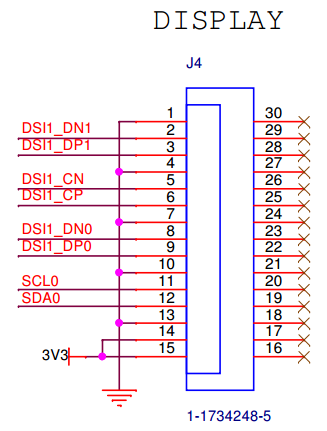
\includegraphics[width=2.5 in]{display}
	\caption{Schematic of Display}
	\label{fig:display}
\end{figure}

\begin{figure}[!htbp]
	\centering
		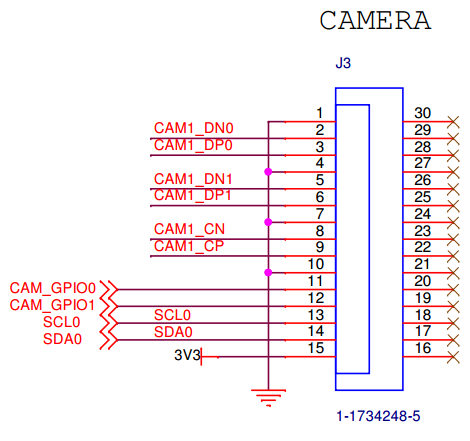
\includegraphics[width=2.5 in]{camera}
	\caption{Schematic of Camera Port}
	\label{fig:camera}
\end{figure}

\begin{figure}[!htbp]
	\centering
		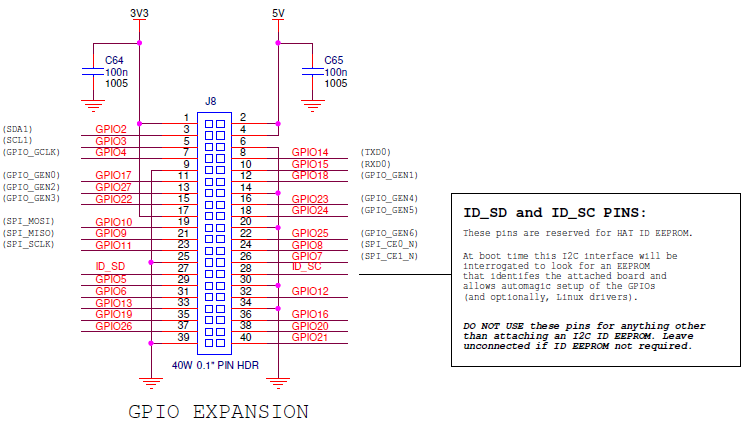
\includegraphics[width=2.5 in]{gpioexpansion}
	\caption{Schematic of GPIO Expansion}
	\label{fig:gpioexpansion}
\end{figure}

\begin{figure}[!htbp]
	\centering
		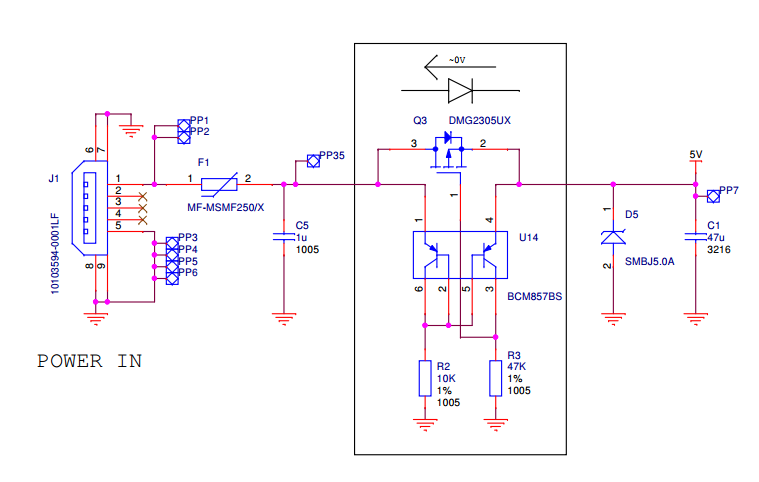
\includegraphics[width=2.5 in]{powerin}
	\caption{Schematic of Power Input}
	\label{fig:powerin}
\end{figure}

\begin{figure}[!htbp]
	\centering
		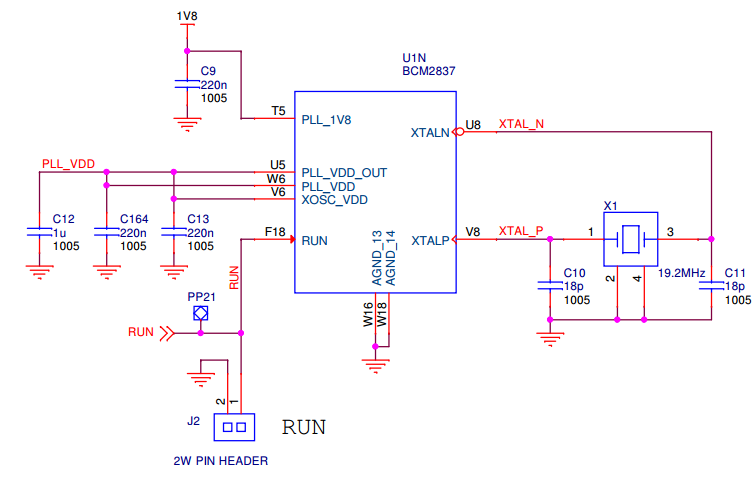
\includegraphics[width=2.5 in]{run}
	\caption{Schematic of RUN}
	\label{fig:run}
\end{figure}

\section{Raspberry Pi Camera Module}

The PiCamera is a camera module for Raspberry Pi that allows the users to capture still photos and record videos in high definition. A camera port on the microcomputer is available for this device. In this port, the camera is connected while Pi is still switched off and once it is connected to the board, the devices are switched on. The camera software is available on the Raspberry Pi Configuration Tool. Python3 is utilized in order to preview the camera. Figure~\ref{fig:code} shows the code to be executed in order to allow the preview of the camera.~\cite{camers}

\begin{figure}[!htbp]
	\centering
		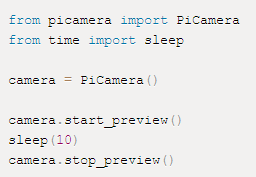
\includegraphics[]{code}
	\caption{Code for Camera  Preview}
	\label{fig:code}
\end{figure}

\section{Virtual Network Computing}
Virtual Network Computing (VNC) is a graphical sharing system on a desktop that allows remote access and control of a desktop interface of on device from another. The events from the controller such as keyboard and mouse are transmitted to the screen over the network from the remote host. 
	On the Raspberry Pi, it is necessary to install the TightVNC package in order to utilize this system. To install this package, the code  \textsl{sudo apt-get install tightvncserver} is used. Running the TightVNC Server would prompt the user to input the password \textsl{tightvncserver}. From the terminal, VNC is started. A session on VNC display one with full HD resolution is written as \textsl{vncserver :1 -geometry 1920x1080 -depth 24}.
	In order to run the VNC server on the Pi, a command on a file is necessary. The shell script \textsl{#!/bin/sh (next line) vncserver :1 -geometry 1920x1080 -depth 24 -dpi 96} is to be created. By inputting the code \textsl{chmod +x vnc.sh}, the shell script with filename vnc.sh is made executable. In order to run the file at any time, the code \textsl{./vnc.sh} is executed.
	The procedure mentioned above is the initialization of VNC on the Pi module. With this, a VNC client on the personal computer is needed in order to connect the computer to the VNC server and have control of it.~\cite{vnc}
	
\section{IP Address}
	Internet Protocol (IP) Address is an address that is used to identify a unique device over an IP network. It is a core in network design as it is a Network Foundation service. It provides the foundation of other network and user services and it allows the interaction of devices within the network.~\cite{cisco}
	Raspberry Pi 3 model B is connected to a Local Area Network. Hence, as any device connected to a LAN, Pi is assigned a unique IP address. IP address is vital information in connecting the Pi to another machine using VNC. The code \textsl{hostname –I} reveals the IP Address of the Pi using the terminal.
		





\section{Design Reference}

\begin{figure}[!htbp]
	\centering
		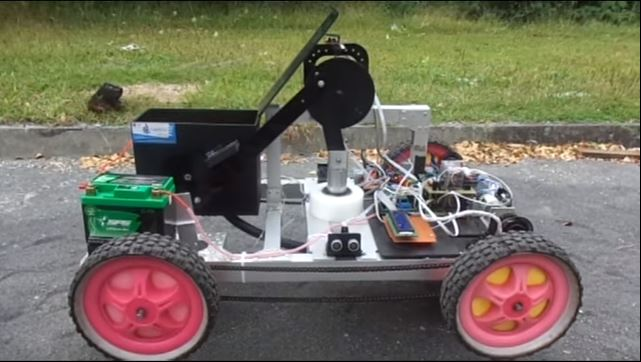
\includegraphics[width=0.5\textwidth]{Capture}
	\caption{Design Reference for The Corn Planting Robot}
	\label{fig:reference}
\end{figure}

Figure \ref{fig:reference} shows the researchers’ design reference for the corn planting robot. The design was found online (youtu.be/QooHpnYLj1w) which is uploaded by user named Luthfi Hasni. The design uses a PIC or a Programmable Integrated Circuit to control the robot. It uses several sensors as its navigation system. Besides from the 2 motors that controls the wheels of the robot, it has a third motor that controls the boring of the soil and the sowing of the cord seeds at the same time. 

\section{Design and Dimensions}

\begin{figure}[!htbp]
	\centering
		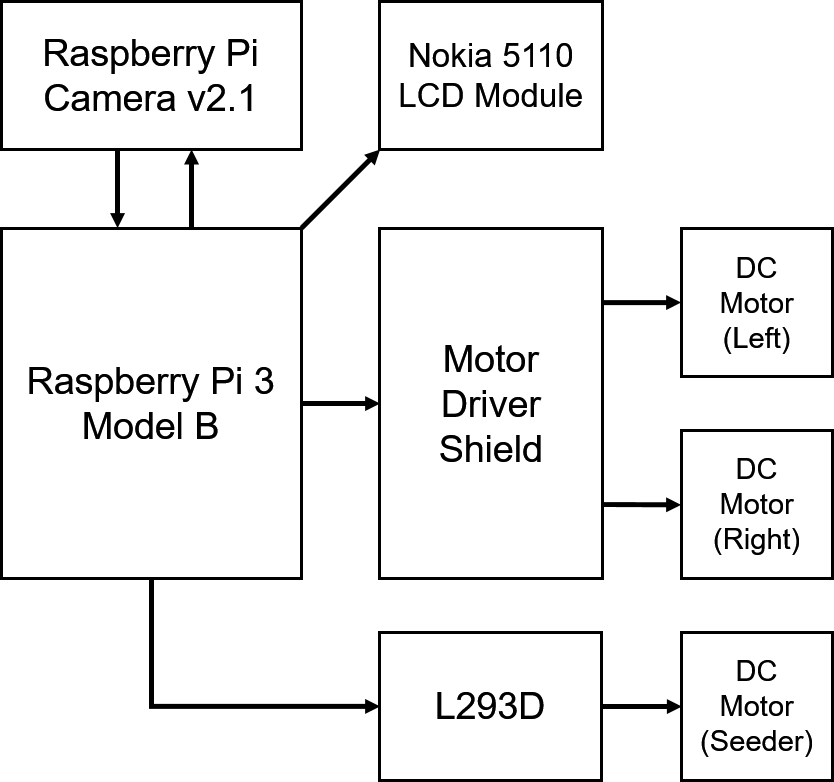
\includegraphics[width=0.5\textwidth]{Design}
	\caption{System Design Diagram}
	\label{fig:Design}
\end{figure}

\begin{figure}[!htbp]
	\centering
		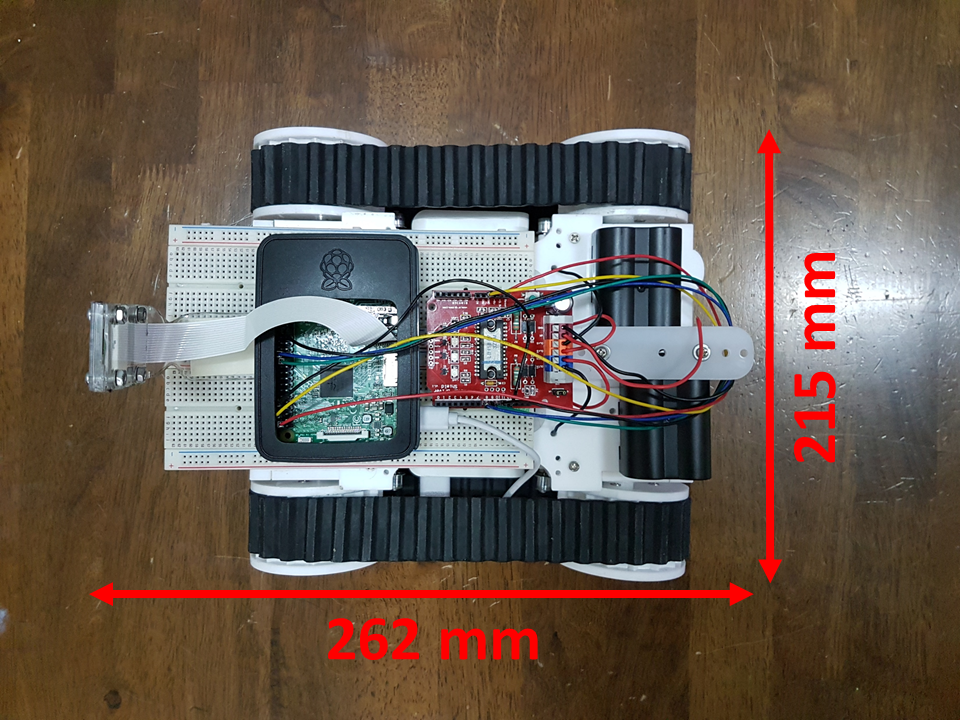
\includegraphics[width=0.5\textwidth]{2}
	\caption{Top View of the Corn Planting Robot and its Dimensions}
	\label{fig:1}
\end{figure}

\begin{figure}[!htbp]
	\centering
		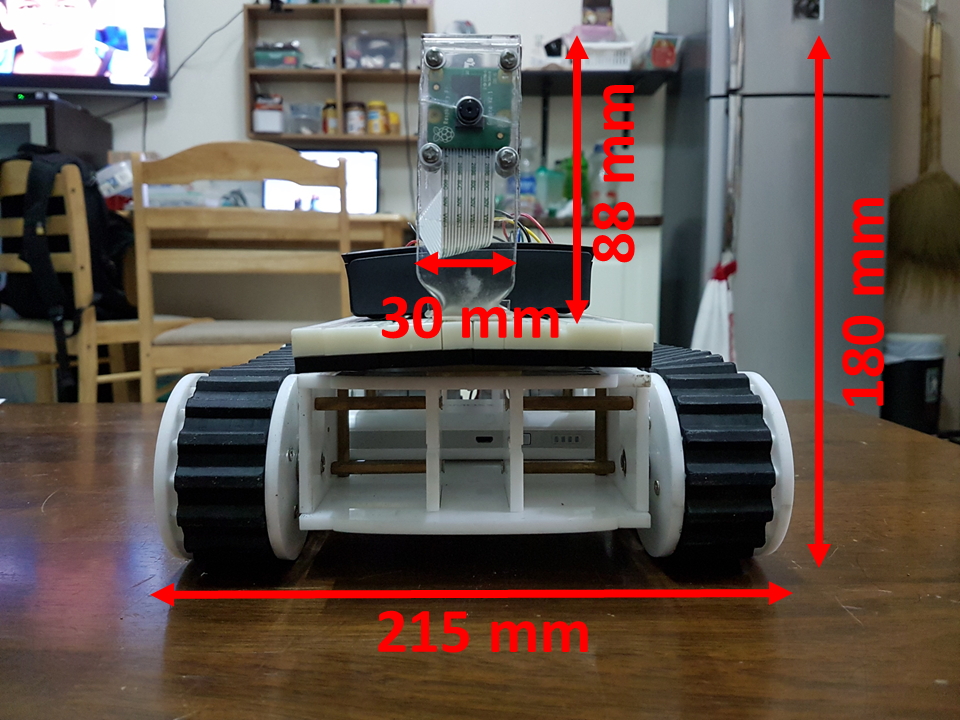
\includegraphics[width=0.5\textwidth]{3}
		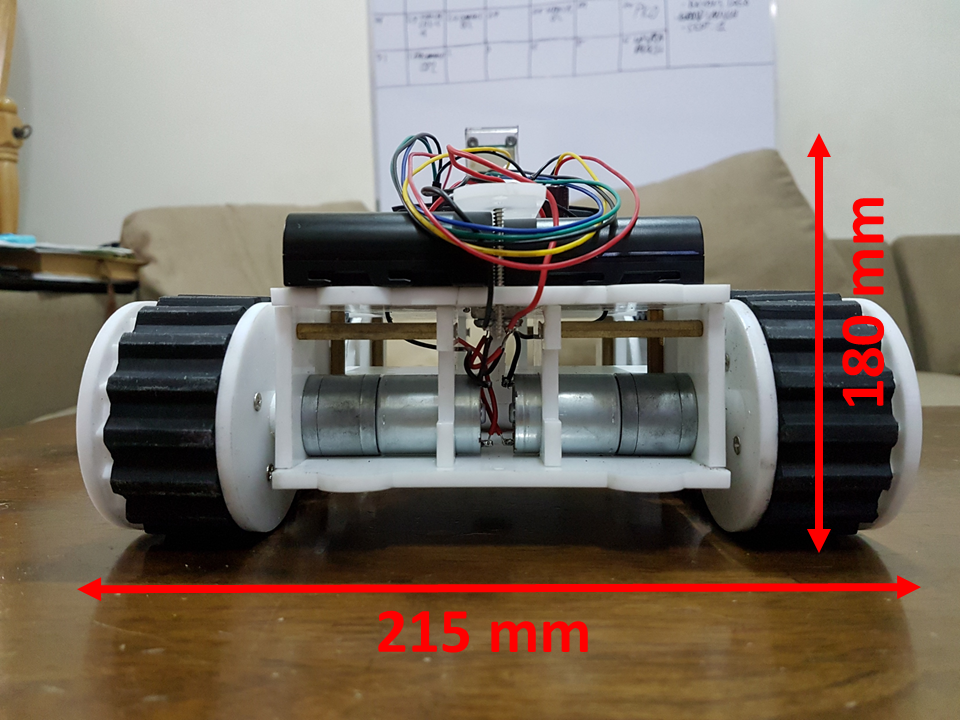
\includegraphics[width=0.5\textwidth]{4}
	\caption{Front and Back View of the Corn Planting Robot and its Dimensions}
	\label{fig:2}
\end{figure}

\begin{figure}[!htbp]
	\centering
		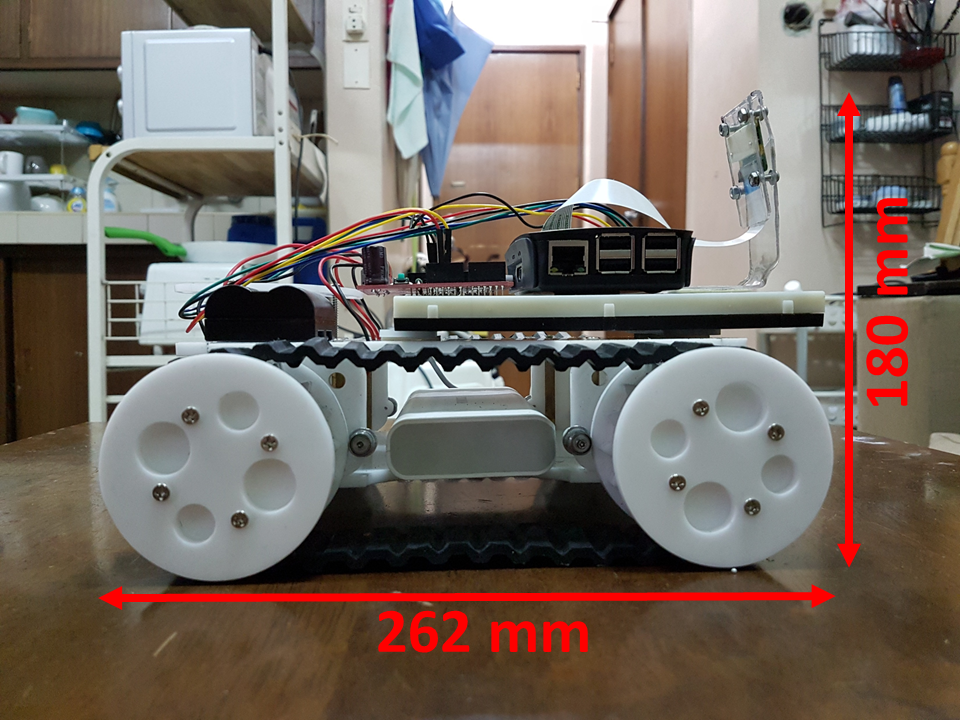
\includegraphics[width=0.5\textwidth]{5}
		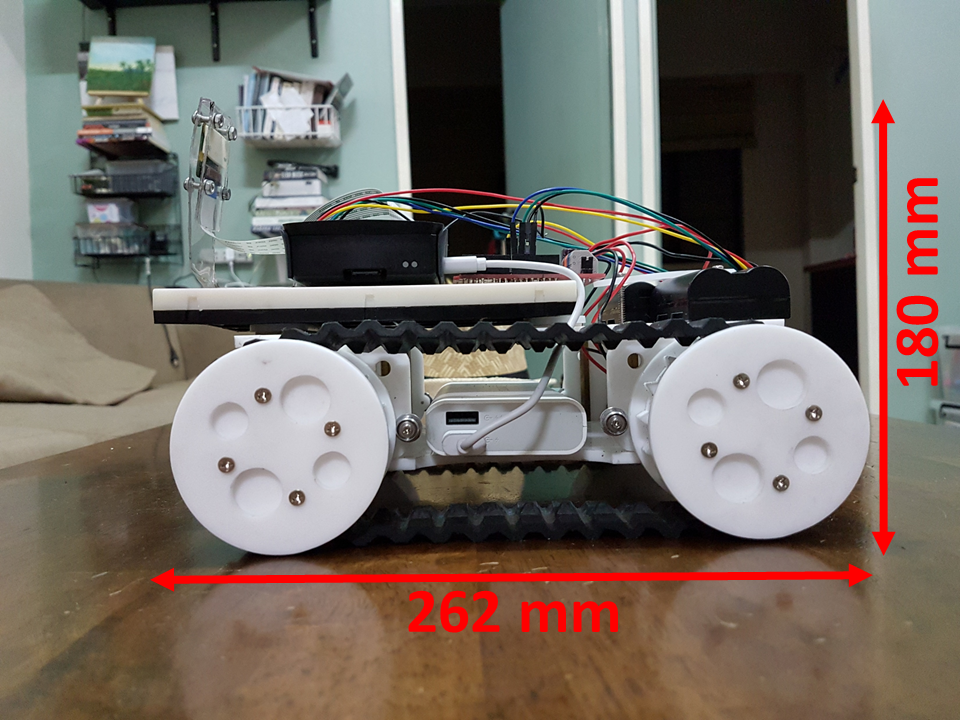
\includegraphics[width=0.5\textwidth]{6}
	\caption{Left and Right Side View of the Corn Planting Robot and its Dimensions}
	\label{fig:3}
\end{figure}

Portability is one of the main considerations of the robot’s design. Figures \ref{fig:1} - \ref{fig:3} shows the design and dimensions of the corn planting robot. The figures show that the researchers’ robot is much smaller compared to the design reference. The robot has a length of 262 mm, a width of 215 mm, and a height of 180 mm.

\section{Components}
\begin{figure}[!htbp]
	\centering
		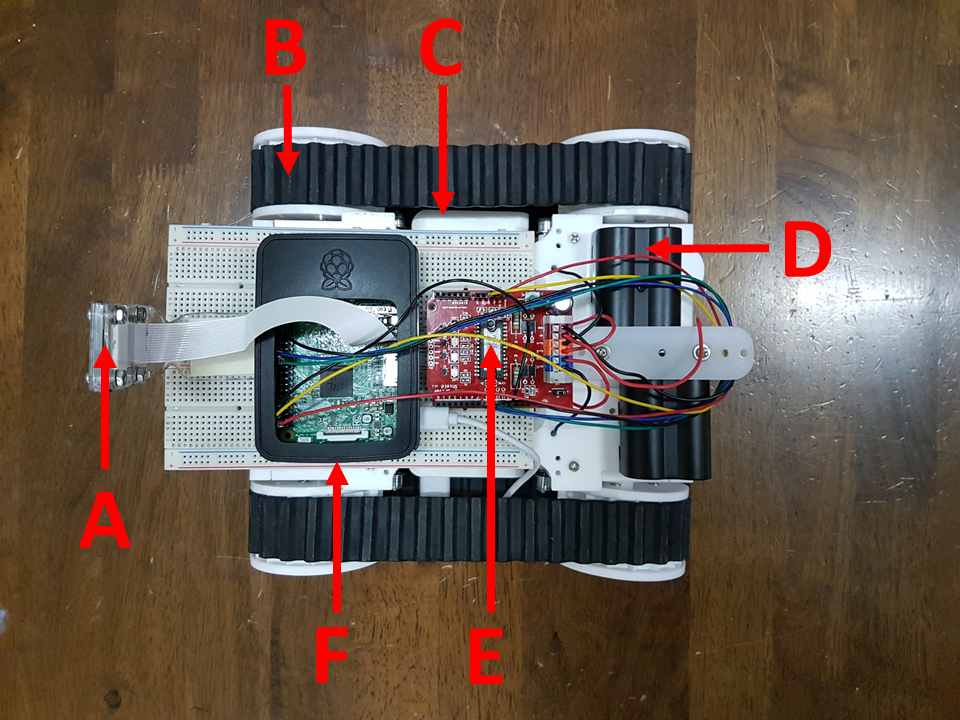
\includegraphics[width=0.5\textwidth]{1}
	\caption{Top View of the Corn Planting Robot with its Main Components Pointed Out}
	\label{fig:4}
\end{figure}

As seen on Figure \ref{fig:4}, part B is the continuous track of the robot. The researchers chose to use a continuous track for the robot since it is more suitable to be used on off-road environments on which corn in planted. The continuous track will help on the slip of the robot on the soil and help with the mobility of the robot.  The robot uses a 6V DC geared motor which controls the continuous track (B) which makes the robot move. Two 7.4 V battery packs (D) that is connected in parallel is used to supply voltage to the motors.  The motors and the battery packs (D) are then connected to the motor driver shield (E) which controls the direction of the motors individually thereby controls the movement of the whole robot. The motor driver shield is connected to the Raspberry Pi 3 Model B (F). The Raspberry Pi is the main processing unit of the robot. It is responsible for the image processing, remote connection, and the control of the motor driver shield (E). For the image processing, the researchers’ used the Raspberry Pi Camera v2.1 (A). We used the Raspberry Pi Camera for it allows the robot to utilize the GPU (Graphical Processing Unit) of the Raspberry Pi, which makes the image processing faster and decrease the processing load on the main processing unit. Lastly, the Raspberry Pi is then powered separately by a power bank.

	The researchers’ decided to use the Raspberry Pi instead of PIC or Arduino and other development boards due to its high processing ability, especially on image processing. PIC and Arduino are more suitable for applications that uses analog sensors or is more focused on hardware projects while the Raspberry Pi is more suitable for software processing. Since the corn planting robot would use computer vision to navigate across the corn field, the Raspberry Pi is more suitable for this kind of application. With a dedicated camera module that is directly compatible and can be easily set up, and a GPU or a Graphical Processing Unit, the Raspberry Pi can do image processing a lot faster which would allow the robot to do real time image processing and navigate across the field at the same time.
